\documentclass[10pt]{article}
\usepackage[T1]{fontenc}
\usepackage{lmodern,amsmath,amssymb,graphicx,hyperref}
\usepackage[margin=.74in]{geometry}
\setlength{\parindent}{0pt}\setlength{\parskip}{7pt}
\begin{document}
\begin{center}{\Large Actual single-anchor odd first-jet cancellation}\\[4pt]
Local continuation --- 15 November 2026\end{center}
\textbf{Result.} The preceding generic parity control is now specialized to
the actual denominator, geometric approximation, numerator and normalization.
With one retained anchor and matching class ports, every admissible odd
moment has zero first-jet coefficient in the actual right factor. This is a
local coefficient identity, not disappearance of a whole mode
[pcc:unverified].

\textbf{Exact setting.} Let $i<u\le a$, retain node $t=-2^i$ and set
$m_j=1$ for $j=i$, zero otherwise. Let $r<2^u$ and use the actual matching
class port $r$ as column. The mask contains $i$. Product reduction uses this
actual membership and these explicit multiplicities; no favorable denominator
is supplied [pcc:unverified].

\textbf{Constructed slopes.} The actual node and anchor slopes are
\[
 -c,\quad+c,\qquad c=\frac{2^u}{2^i}=2^{u-i}.
\]
Applying the actual constant-coefficient map in $Z$ to denomRows gives
\[
 D(H,0)=(1-cH)(1+cH)=1-c^2H^2.
\]
The chart term vanishes at $Z=0$. The proof handles the integer pole,
residue-class representative, anchor mask, scalar signs and natural exponent
subtraction explicitly [pcc:unverified].

\textbf{Actual geometric coefficients.} Mapping the actual finite sum
$G_k=\sum_{n<k}(1-D)^n$ at $Z=0$ yields
\[
 G_k(H,0)=\sum_{n<k}(c^2H^2)^n.
\]
Hence $[H^{2s+1}Z^0]G_k=0$ for all natural $s,k$. This uses the previously
proved generic odd-coefficient identity only after the actual specialization
has been established. The empty sum remains included [pcc:unverified].

\textbf{Actual right factor.} The matching-port actual row numerator has
$N(0)=0$ and $[Z^1]N=1$. Therefore the actual approximation satisfies
\[
 [Z^1]\bigl([H^{2s+1}](N G_k)\bigr)=0.
\]
The actual outer normalization is multiplication by $2^{-(2s+1)}$.
For every admissible label $2s+1<k$, the final theorem proves
\[
 [Z^1]R_{(r,2s+1),r}(Z)=0.
\]
No normalization or label condition is omitted [pcc:unverified].

\textbf{Evidence.} Accepted081 contains384 local theorem statements including
parent376, eight new; exit0 with no warnings or sorryAx. Receipt041 binds
exact source, raw compiler output and exit. Central printed dependencies are
standard. The evidence is outside shared Transport53/57/fresh and remains
unsigned, defaultnot\_covered [pcc:unverified].
\newpage
\begin{center}{\Large Scope and discriminating controls}\end{center}
\begin{center}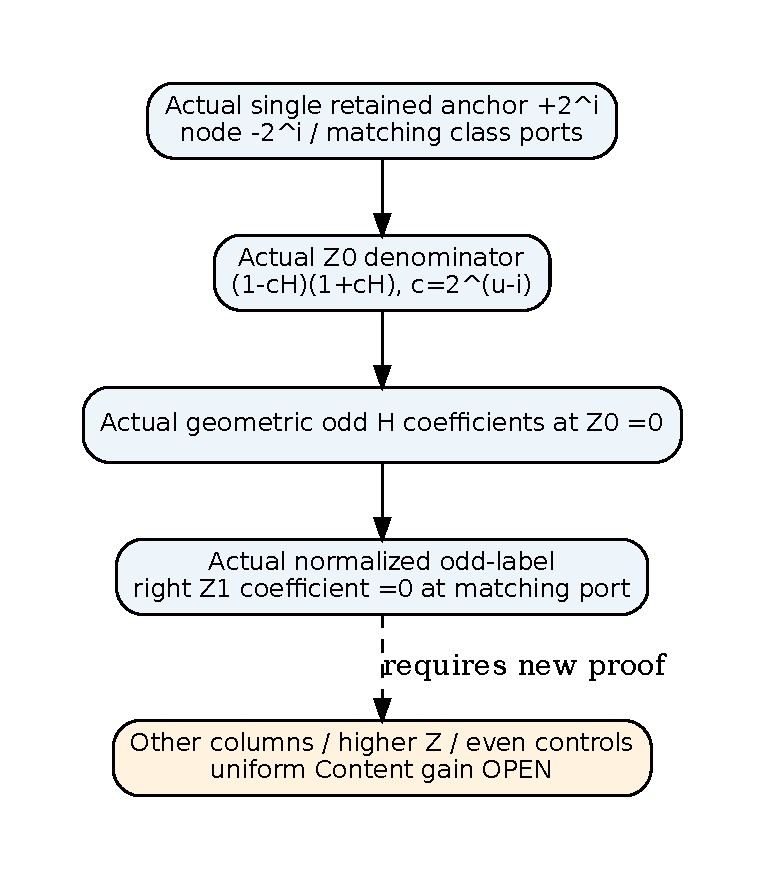
\includegraphics[height=3.1in]{actual-parity-dependencies-001.pdf}\end{center}
\textbf{What was established.} This is an actual polynomial coefficient
identity for a specific retained multiplicity profile and matching ports.
It extends the generic symmetric-pair control without assuming that the
actual denominator has the desired shape. Standard polynomial maps, finite
sums and coefficient products are reused; no arithmetic novelty is claimed
[pcc:unverified].

\textbf{What remains unproved.} The right polynomial can have nonzero higher
$Z$ coefficients. Other columns may have nonzero first jets. Thus this proof
does not remove an entire mode, increase its uniform weight, reduce total
inventory or prove an asymptotic runtime gain. All $2^u k$ labels remain
charged until actual uniform support or valuation results justify a change
[pcc:unverified].

\textbf{Next exact control.} PROTOCOL-012.md fixes $a=u=2$, $i=0$, $k=2$,
$r=0$, column $y=2$ and odd label $b=1$ with the same single-anchor profile.
The retained bit condition holds. The prospective prediction is first-jet
coefficient $-8/9$; it is not yet a proved or measured result. Prove or refute
it from the actual formulas, then check even-index nonzero and higher-$Z$
controls before any uniform conclusion [pcc:unverified].

\textbf{Failures and provenance.} Failed079 and080 are retained with raw
sources, compiler output and exits. They exposed slope-name/sign and namespace
issues; they are not mathematical counterexamples. Prior source reviews pin
the actual polynomial definitions and standard Mathlib identities. KB tools
and wrapper executable remain unavailable; exact primary/repository fallback
is recorded. Parent immutable reports, claims and ledger bytes remain exact
[pcc:unverified].

\textbf{Remaining interfaces.} Original packet metadata and child budgets,
complete preparation, control, index, array, trace and memory costs, actual elliptic
relation, public finder, field/scalar extraction, retries and expected bit
cost remain open. No native timing, scaling, paid/cloud or attack campaign
was launched. The subordinate PR watcher stays paused, and no protected
history reconciliation is attempted [pcc:unverified].
\end{document}
